\chapter{Einführung} % (fold)
\label{cha:einführung}

\emph{„How people work is one of the best kept secrets in America.“} (Wellman, D. zitiert nach \citep{Suchman95}).

Diese Aussage David Wellmans diente Lucy Suchman in den 90er-Jahren des 20. Jahrhunderts als Motivator für ihre Forschung über die Natur menschlicher Arbeit im Computerzeitalter und deren Unterstützung durch neue Technologien. Ihre Arbeiten und viele andere (etwa \citep{Schmidt92} oder \citep{Sachs95}) argumentieren für eine stärkere Berücksichtigung der Rolle des Menschen im Arbeitsprozess.

Wellman spielt mit diesem Zitat auf die oft auftretende Diskrepanz zwischen der (niedergeschriebenen) Definition eines Arbeitsablaufs und dessen tatsächlicher Umsetzung in der konkreten betrieblichen Umgebung an.

Der Druck in der heutigen Geschäftswelt, bestimmte Qualitätskriterien garantiert erfüllen zu können, hat zu einer beinahe flächendeckenden Verbreitung von Qualitätszertifizierungen geführt. Die bekanntesten Vertreter dieser Zertifizierungen sind wohl die Standards aus der Familie der ISO 9000 Normen \citep{ISO05}. In der ISO 9001-Norm \citep{ISO00}, in der die Anforderungen an Qualitätsmanagement-Systeme definiert sind, ist festgeschrieben, dass eine prozessorientierte Organisation eine der Voraussetzungen für erfolgreiches Qualitätsmanagement ist. Ein wesentliches Merkmal einer prozessorientierten Organisation ist, dass ihre organisationalen Prozesse — also ihre Arbeitsorganisation und -abläufe — bekannt, benannt und definiert sind. 

Die Unterschiede zwischen festgeschriebenen und gelebten Arbeitsabläufen wurde schon 1978 von Argyris und Schön \citep{Argyris78} beschrieben. Mit der Unterscheidung zwischen „\emph{espoused theories}“ (= \emph{die offiziell veröffentlichten Theorien über Arbeit}) und den „\emph{theories-in-use}“ (= \emph{die tatsächlich handlungsleitenden Theorien}) wurden dieser Gegensatz auch explizit benannt. Sachs \citep{Sachs95} beschreibt das gleiche Phänomen und unterscheidet zwischen dem „\emph{explicit organisational view}“ und dem „\emph{tacit organisational view}“ auf Arbeit. Sie beschreibt damit einerseits eine explizit formulierte und statische Sicht auf Arbeit und andererseits eine informelle, im Fluss befindliche und zum Zeitpunkt der Betrachtung nirgendwo niedergeschriebene Sicht auf Arbeit. Letztere kann lediglich aus der Analyse der tatsächlichen Arbeitsabläufe gewonnen werden kann, die den Tätigkeiten zugrunde liegenden Annahmen („theories-in-use“ \citep{Argyris78}) sowie deren vom Arbeitenden konkret wahrgenommene organisationale Rahmenbedingungen bleiben allerdings verborgen — die Frage nach dem „Warum?“, die die Form des konkreten Arbeitsablaufs motiviert, kann nicht unmittelbar beantwortet werden.

Wie Sachs verdeutlichen auch Wellman sowie Argyris und Schön, dass das zweitgenannte Verständnis von Arbeit nicht explizit niedergeschrieben und formal definiert ist -- also nur in den Köpfen der beteiligten Individuen existiert. Wenn „Arbeit“ oder die ihr zugrunde liegenden Annahmen aber nicht expliziert sind und die beteiligten Personen unter Umständen unterschiedliche Sichtweisen auf die gemeinsame „Arbeit“ haben, kann eine Veränderung der „Arbeit“ selbst oder der Umgebung, in der sie durchgeführt wird, zu schwerwiegenden Problemen führen (wie z.B. von \citet{Nonaka95}, \citet{Krogh00} oder \citet{Gerson86} beschrieben). Der Begriff „Veränderung“ deckt dabei nicht nur tiefgreifende organisatorische Änderungen im Unternehmen ab, sondern durchaus auch vordergründig „marginale“ Änderungen wie z.B. die Einstellung neuer Mitarbeiter oder dem Einsatz eines neuen Werkzeugs \citep{Olesen03}. Daraus kann geschlossen werden, dass potentiell „problematische“ Situationen häufig auftreten können. 

„Problematische“ Situationen sind dabei all jene Situationen, in denen die Zielerreichung erschwert wird, weil die dazu notwendigen Schritte entweder unklar sind oder nicht operationalisiert werden können. Im Kontext der obigen Aussage bedeutet dies, dass durch eine organisationale Veränderung neue Arbeitsschritte notwendig werden bzw. die bisherigen nicht mehr durchgeführt werden können oder angemessen sind. Beim Auftreten einer derartigen Veränderung ist daher eine erneute Planung bzw. Abstimmung der zur Zielerreichung notwendigen Arbeitsschritte notwendig. \citet{Fujimura87} unterscheidet in diesem Zusammenhang zwischen zwei Formen von Arbeit — der „Produktion“ („\emph{production}“) und der „Artikulation“ („\emph{articulation}“), wobei letztere alle Tätigkeiten umfasst, die die Umsetzung bzw. Aufrechterhaltung der „Produktion“ ermöglichen.

„Artikulation“ ist ein integraler Bestandteil von Arbeit \citep{Strauss85}. Mit der Komplexität der „Produktion“ steigt auch der Aufwand der dazu notwendigen „Artikulation“ an \citep{Strauss88}. Die Komplexität steigt hier mit der Anzahl der benötigten Arbeitsschritte, den dazu benötigten Kompetenzen und der Anzahl der involvierten Personen. Je komplexer („problematic“) eine Interaktion ist, desto notwendiger wird nach \citep{Strauss88} eine explizite Beschäftigung mit dem Vorgang der Artikulation. Werden Tätigkeiten in diesem Rahmen bewusst durchgeführt, so spricht man von \emph{expliziter} „Articulation Work“ \citep{Strauss88} \citep{Fjuk97}. Die Abstimmung von Tätigkeiten, die ständig während der Zusammenarbeit unbewusst ausgeführt wird, wird als \emph{implizite} „Articulation Work“ bezeichnet \citep{Fjuk97}. 

Letztgenannte Art ist es auch, die von Arbeitenden „automatisch“ zur Anwendung gebracht wird, sobald Änderungen in der Arbeitsumgebung auftreten \citep{Strauss88}. Implizite „Articulation Work“ stößt aber an ihre Grenzen, wenn die Arbeitssituation als „problematisch“ \citep{Strauss88} oder „komplex“ \citep[][S. 23f]{Schmidt90} wahrgenommen wird. Es wird dann notwendig, dezidierte Abstimmungs-Aktivitäten anzustoßen, also explizite „Articulation Work“ durchzuführen.

Nicht bekannte, falsche oder zurückgehaltene Information über die „Production Work“ erschweren die „Articulation Work“ oder machen sie unmöglich \citep{Fujimura87}. Dies hat jedoch nicht nur negative Auswirkungen auf die „Production Work“ sondern verhindert auch eine tiefergehende Beschäftigung mit der aktuellen Arbeitspraxis und eine potentielle Verbesserung derselben \citep{Argyris78}. Erfolgreiche Artikulation ist damit nicht nur eine Voraussetzung für eine funktionierende Produktion sondern ermöglicht auch organisationale Veränderungen im Sinne eines organisationalen Lernprozesses (z.B. \citep{Kim93} oder \citep{Firestone03a}).

Eine methodische und technische Unterstützung kann Artikulation ermöglichen oder deren erfolgreichen Ablauf erleichtern (z.B. beschrieben bei \citet{Schmidt92}, \citet{Simone99}, \citet{Jorgensen04} oder \citet{Baker07}). Die konkrete Unterstützung von „expliziter Articulation Work“, also beim Auftreten von Situationen, in denen Arbeit von den Beteiligten als so problematisch oder unklar wahrgenommen wird, dass eine Durchführung als nicht (mehr) möglich erscheint und eine explizite Beschäftigung damit notwendig ist, ist jedoch ein in der bisherigen Forschung weitgehend unadressiertes Feld. Aus diesem Grund widmet sich die vorliegende Arbeit der Bearbeitung folgender Zielsetzung: 

\fbox{\parbox{13cm}{\label{zielsetzung}\textbf{In der vorliegenden Arbeit sind die methodischen und technischen Möglichkeiten zur Ermöglichung und Unterstützung von expliziter Articulation Work zu ergründen, die gewonnenen Erkenntnissen in einem Werkzeug umzusetzen und dessen Auswirkungen auf die Interaktion zur Verbesserung der Production Work zu bewerten.}}}

\section{Forschungsfragen} % (fold)
\label{sec:forschungsfragen}

Aus der oben formulierten Zielsetzung müssen zur strukturierten Bearbeitung detaillierte Fragestellungen abgeleitet werden. Es lassen sich folgende Fragestellungen identifizieren:

\begin{enumerate}
	\item Wie kann explizite Articulation Work ermöglicht und unterstützt werden?
		\begin{enumerate}
			\item Durch welche Aktivitäten zeigt sich Articulation Work im Arbeitsprozess?
			\item Welche Rahmenbedingungen ermöglichen bzw. begünstigen Articulation Work?
			\item Wie können die in 1a identifizierten Aktivitäten unterstützt werden?
			\item Wie können die in 1b identifizierten Rahmenbedingungen und die in 1c identifizierten Anforderungen in einer Methodik umgesetzt werden?
		\end{enumerate}
	\item Was muss ein Werkzeug zur Unterstützung von expliziter Articulation Work leisten?
		\begin{enumerate}
			\item Welche Anforderungen an ein Werkzeug ergeben sich aus der in 1d entwickelten Methodik?
			\item Wie können diese Anforderungen technologisch umgesetzt werden?
		\end{enumerate}
	\item Inwiefern unterstützt das entwickelte Werkzeug die Durchführung von Articulation Work?
		\begin{enumerate}
			\item Wie kann die Unterstützungsleistung bewertet werden?
			\item Welche Auswirkungen auf die Interaktion hat die Anwendung von Methodik und Werkzeug?
		\end{enumerate}
\end{enumerate}

Diese Fragestellungen müssen im Rahmen der Durchführung dieser Arbeit beantwortet werden. In Kapitel \ref{cha:schlussbetrachtungen} ist die globale Zielsetzung wieder aufzugreifen und einer abschließenden Bewertung hinsichtlich ihrer Erfüllung zu unterziehen. 

% section forschungsfragen (end)

\section{Anmerkung zur wissenschaftstheoretischen Grundlage}
\label{sec:wissenschaftstheoretische_grundlage}

Dieser Arbeit basiert auf den Annahmen des Konstruktivismus. Die Grundannahme, auf der die weiteren Ausführungen basieren, ist die Exisitenz von individuellen „Realitäten“, die aufgrund der Wahrnehmung eines Indivuduums, seiner Erfahrungen und Grundannahmen der Welt gebildet werden. Die Existenz einer objektiv exitierenden „Realität“ wird angenommen (aber nicht paradigmatisch vorausgesetzt). Die individuellen „Realitäten“ stehen insofern in Zusammenhang mit einer objektiven „Realität“, als dass letztgenannte -- gefiltert durch individuelle Wahrnehmung, Erfahrungen und Grundannahmen -- die Grundlage der erstgenannten bildet.

Ziel dieser Arbeit ist es aus dieser Perspektive, individuelle Realitäten abzustimmen, also die filternden Faktoren der individuellen Wahrnehmung so zu beeinflussen, dass die für eine erfolgreiche Zusammenarbeit relevanten Bereiche der objektiven „Realität“ zu ähnlichen Abbildungen in der individuellen „Realität“ aller Beteiligten führen.

% chapter einführung (end)
\section{Aufbau der Arbeit} % (fold)
\label{sec:aufbau_der_arbeit}

In diesem Abschnitt wird die Struktur der Arbeit auf globaler Ebene dargestellt. Zusätzlich wird der inhaltliche Aufbau der einzelnen Kapitel zueinander in Beziehung gesetzt und so der rote Faden durch die Arbeit transparent gemacht.

Die hier vorgestellte Struktur ist auszugsweise auch am Beginn jedes Kapitels beschrieben und graphisch dargestellt, um die Einordnung der Kapitel in den Gesamtzusammenhang der Arbeit zu erleichtern.

\subsection{Überblick} % (fold)
\label{sub:aufbau_ueberblick}

Die Arbeit gliedert sich inhaltlich in drei große Teile, die durch das Einleitungs- und Schlusskapitel eingerahmt werden.

Teil \ref{prt:grundlagen} behandelt die konzeptuellen Grundlagen der Arbeit und schafft die Argumentationsgrundlage für die Entwicklung des Werkzeugs. Er deckt damit im Wesentlichen die Beantwortung der ersten oben formulierten Forschungsfrage ab. Im Einzelnen umfasst Teil \ref{prt:grundlagen} ein Kapitel über „Articulation Work“ (Fragestellungen 1a und 1b, Kapitel \ref{cha:articulation_work}) und ein Kapitel über „Mentale Modelle“ (Fragestellung 1c, Kapitel \ref{cha:mentale_modelle}). Teil \ref{prt:grundlagen} endet mit einem Kapitel über Methodik der Anwendungsszenarien, in dem beschrieben wird, wie mentale Modelle für die Verwendung für „Articulation Work“ externalisiert und abgestimmt werden können (Fragestellung 1d, Kapitel \ref{cha:methodik}).

Teil \ref{prt:umsetzung} behandelt die Umsetzung des Werkzeugs selbst. Er deckt damit im Wesentlichen die Beantwortung der zweiten oben formulierten Forschungsfrage ab. Das erste Kapitel greift die Ergebnisse des ersten Teils auf und leitet daraus die Anforderungen an das Werkzeug ab (Fragestellung 2a, Kapitel \ref{cha:anforderungen}). In Kapitel \ref{cha:implementierung_Überblick} werden die konzeptuellen Grundlagen für die Implementierung aus dem Kontext von Tangible Interfaces heraus aufgearbeitet. Die Kapitel \ref{cha:input_&_interpretation}, \ref{cha:visualisierung} und \ref{cha:persistierung} beschreiben nacheinander die technische Umsetzung des Werkzeugs -- beginnend von den Eingabekanälen über die Ausgabekanäle bis zu Persistierung der Modelle. Sie beantworten also die Fragestellung 2b. 

Teil \ref{prt:evaluierung} behandelt die Evaluierung des Werkzeugs. Er deckt damit im Wesentlichen die Beantwortung der dritten oben formulierten Forschungsfrage ab. Dabei beginnt Kapitel \ref{cha:konzeptuelle_evaluierung} mit einer konzeptuellen Betrachtung des umgesetzten Systems (also einer theoretischen Einordnung des Werkzeugs auf Basis der Ergebnisse von Kapitel \ref{cha:implementierung_Überblick}, den konzeptuellen Grundlagen der Implementierung). In Kapitel \ref{cha:eval_ueberblick} werden die grundsätzliche Ausrichtung der empirischen Untersuchung und die durchgeführten Evaluierungen beschrieben. Die Kapitel \ref{cha:eval_werkzeug}, \ref{cha:eval_modell} und \ref{cha:eval_aw} beschäftigen sich mit der Ableitung der Hypothesen und deren Prüfung auf den unterschiedlichen Untersuchungsebenen der Arbeit. Dies beginnt mit der Prüfung der grundsätzlichen Verwendung des Systems (Kapitel \ref{cha:eval_werkzeug}), setzt mit der Prüfung der Eignung für die Externalisierung mentaler Modelle fort (Kapitel \ref{cha:eval_modell}) und endet mit der Prüfung der Eignung für „Articulation Work“ selbst (Kapitel \ref{cha:eval_aw}). Die Fragestellungen 3a und 3b sind damit Gegenstand der hier genannten Kapitel.

Der Schlussteil (Kapitel \ref{cha:schlussbetrachtungen}) fasst die Ergebnisse zusammen und spiegelt diese auf die ursprüngliche Zielsetzung zurück.

Die Gesamtstruktur dieser Arbeit ist in Abbildung \ref{fig:img_Einfuehrung_gesamtueberblick} nochmals zusammenfassend dargestellt. Die Beziehungen zwischen den einzelnen Kapiteln sind als Pfeile zwischen den einzelnen Blöcken dargestellt, wobei jeweils der Endpunkt Ergebnisse des Startpunktes als Grundlage für die weiteren Ausführungen verwendet.

\begin{figure}[htbp]
	\centering
		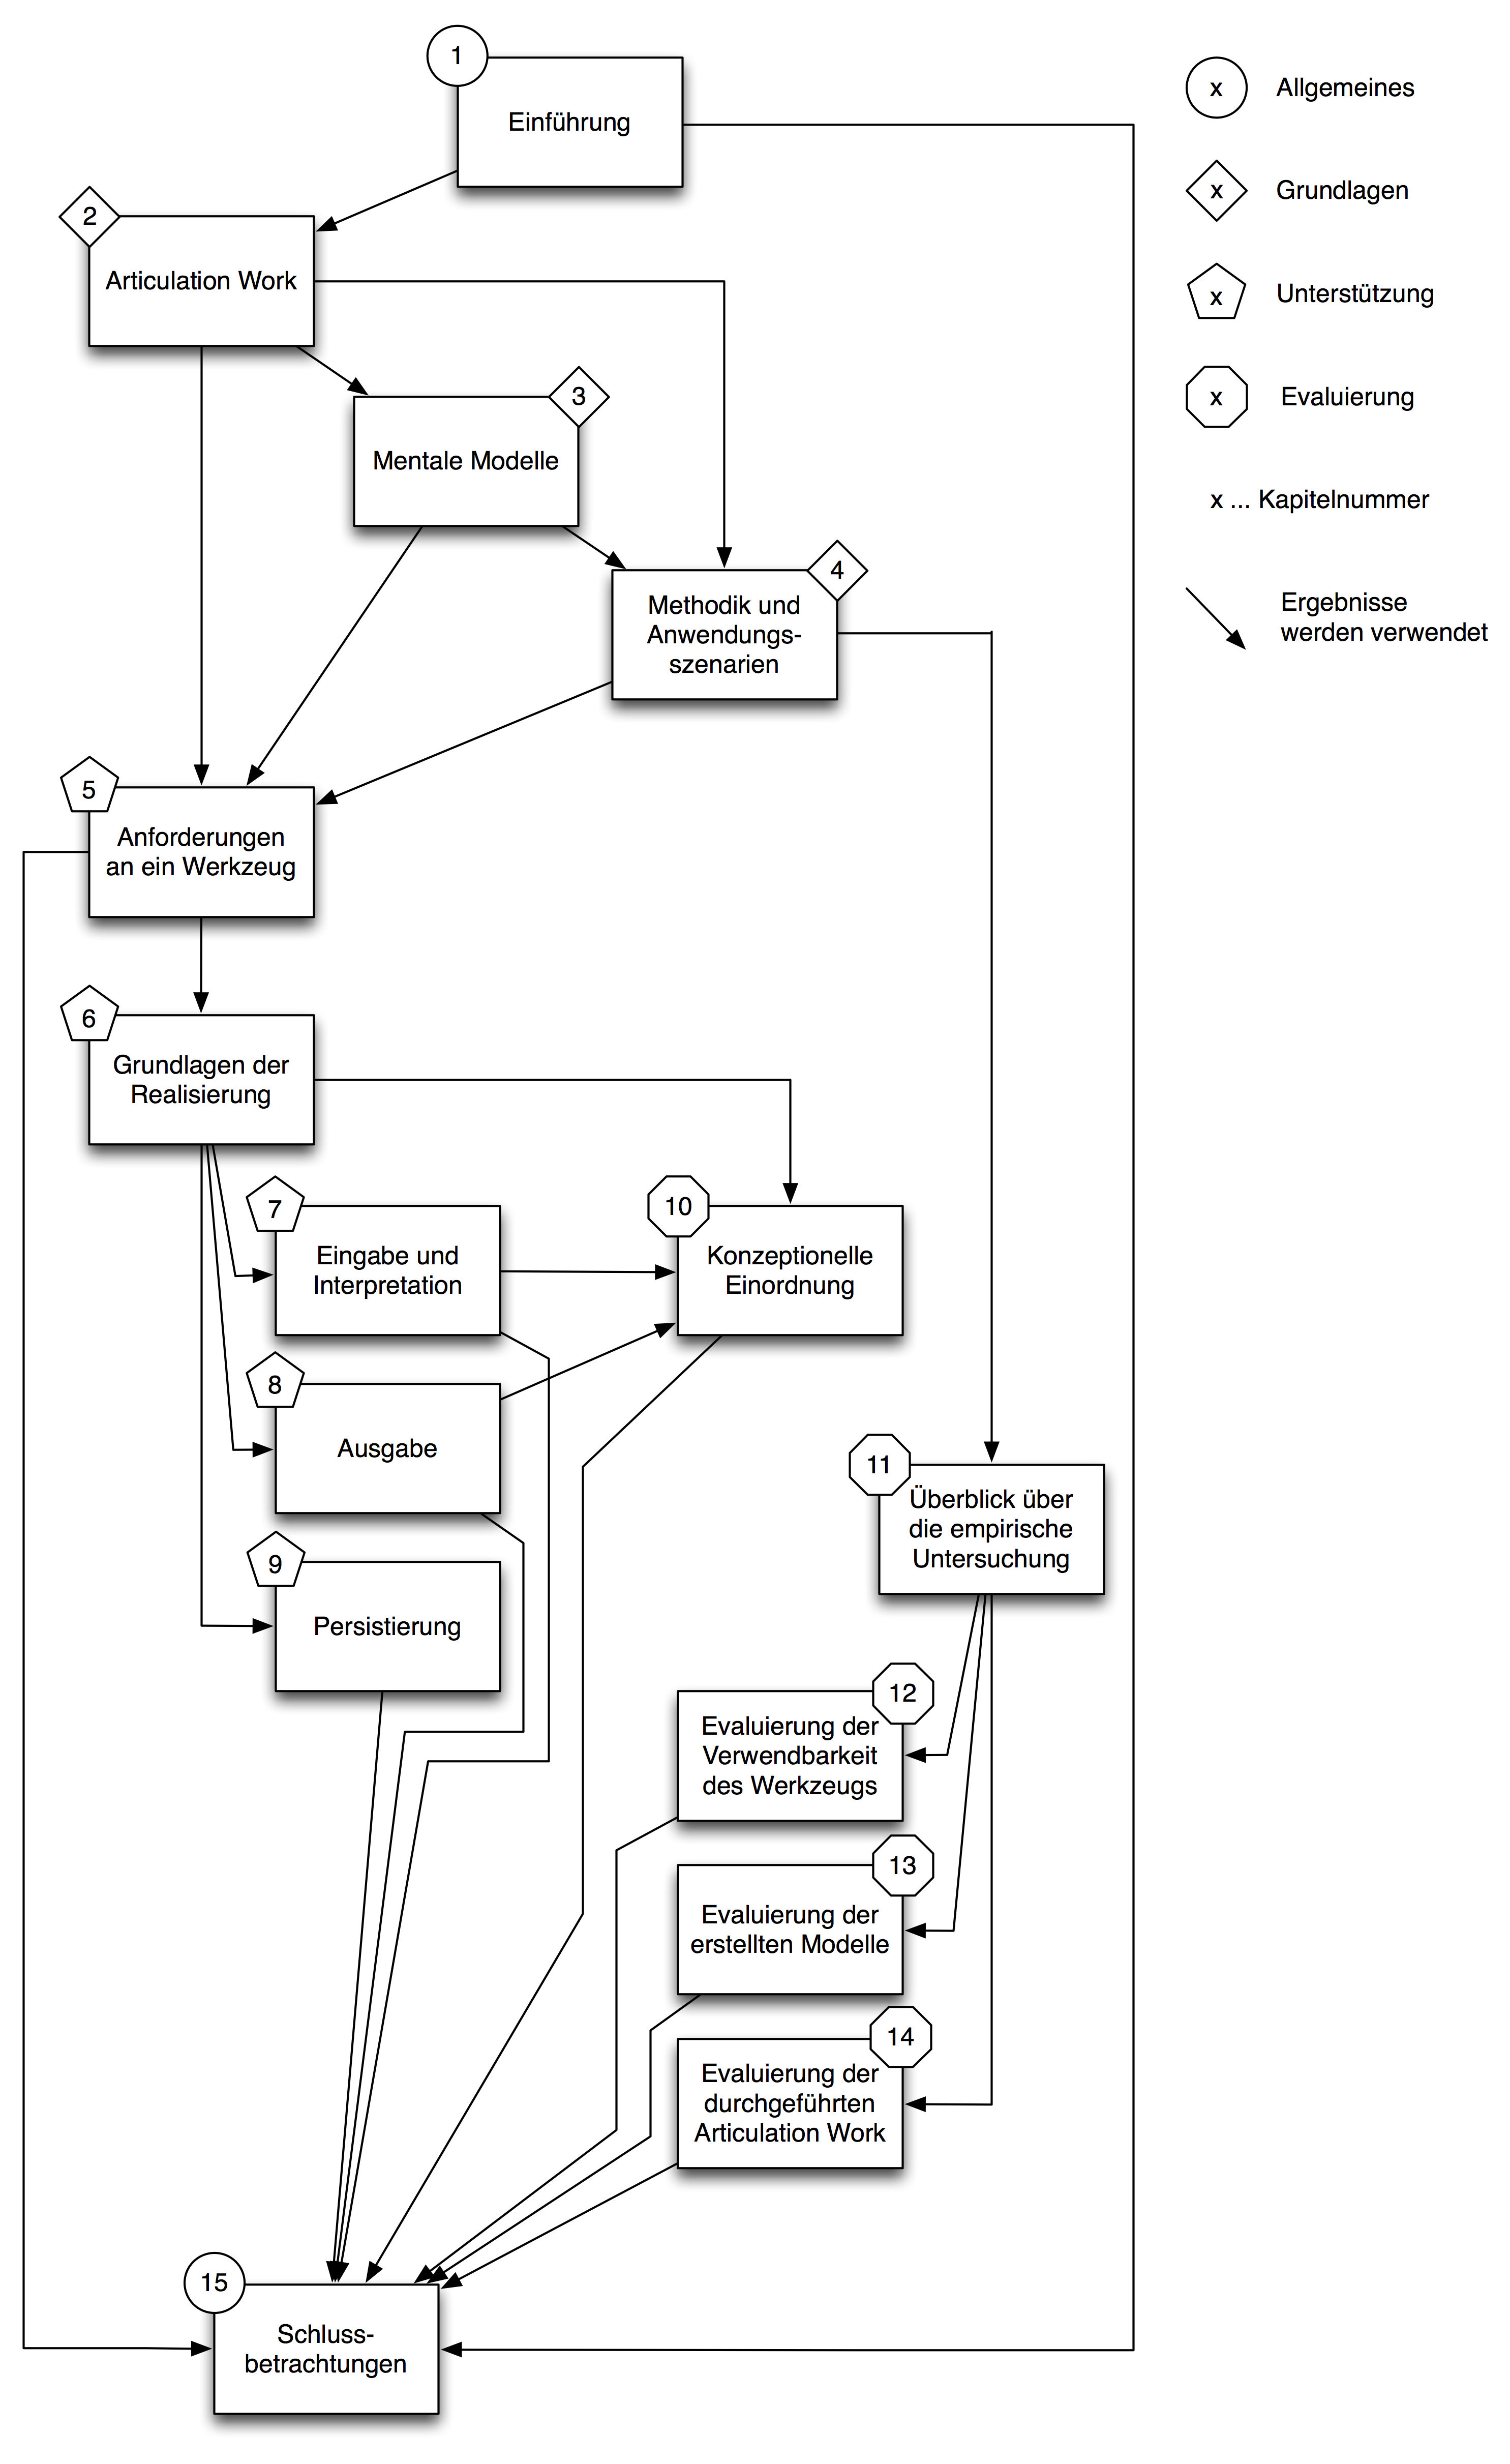
\includegraphics[height=0.9\textheight]{img/Einfuehrung/gesamtueberblick.png}
	\caption{Zusammenhänge zwischen den Kapiteln der Arbeit}
	\label{fig:img_Einfuehrung_gesamtueberblick}
\end{figure}

Anhang \ref{cha:literatur_zum_themengebiet_articulation_work} ist als Ergänzung zu Kapitel \ref{cha:articulation_work} (Articulation Work) zu sehen und stellt die gesamte zu diesem Gebiet erschienene Literatur strukturiert dar.

Anhang \ref{cha:daten_der_empirischen_untersuchung} ergänzt die Evaluierungskapitel in Teil \ref{prt:evaluierung} durch eine Zusammenfassung der im Rahmen der Untersuchung erhobenen Daten.
% subsection aufbau_ueberblick (end)

\subsection{Zusammenfassung der Zusammenhänge -- Ausblick} % (fold)
\label{sub:zusammenhänge}

Dieser Abschnitt stellt die wesentlichen inhaltlichen Zusammenhänge der Arbeit dar und versucht so ein erstes Bild des roten Fadens durch die Arbeit zu vermitteln. Er ergänzt somit die im letzten Abschnitt dargestellte Struktur der Arbeit um eine detaillierte inhaltliche Sicht und fasst das Vorgehen bei der Bearbeitung der in Abschnitt \ref{sec:forschungsfragen} formulierten Forschungsfragen zusammen.

Kapitel \ref{cha:articulation_work} beginnt mit einer generellen Begriffsbestimmung zum Themenfeld Articulation Work. Diese bildet die Grundlage für den nächsten Abschnitt, in dem auf Basis der Literatur geklärt wird, wie sich „Articulation Work“ manifestiert und in welchen unterschiedlichen Ausprägungen sie das tut. Das Ergebnis ist in Abbildung \ref{fig:img_ArticulationWork_aw_conceptual_structure} zusammengefasst und spannt die in dieser Arbeit verwendete Taxonomie auf. In den beiden folgenden Abschnitten wird auf Basis der Literatur dargestellt, was (welche Arbeitsaspekte) Gegenstand von „Articulation Work“ ist und wie „Articulation Work“ unterstützt werden kann (siehe dazu auch Anhang \ref{cha:literatur_zum_themengebiet_articulation_work} für eine Gesamtübersicht über die zu „Articulation Work“ verfügbare Literatur). Schließlich greift der letzte Abschnitt die Ergebnisse der Literaturstudien wieder auf und identifiziert eine konzeptuelle Lücke im Gesamtrahmenwerk -- nämlich die bislang vernachlässigte Rolle des Individuums bei „Articulation Work“ und dessen konkrete Tätigkeiten. Zu diesem Aspekt existieren wenige Aussagen in der Literatur, lediglich Strauss selbst weißt in seinen Arbeiten zu „Articulation Work“ auf die Lücke hin, die entsteht, wenn auf die sozialen und organisationalen Aspekte von „Articulation Work“ fokussiert wird, die individuellen „thought processes“ aber außer Acht gelassen werden.

In Kapitel \ref{cha:mentale_modelle} wird die identifizierte Lücke aufgegriffen und konzeptuell mit dem Erklärungsmodell der mentalen Modelle hinterlegt. Im Kontext von „Articulation Work“ sind mentale Modelle jener Beitrag, den jedes beteiligte Individuum einbringt und der in der Folge Gegenstand der Abstimmung und Aushandlung sein muss, um eine gemeinsame Sichtweise zu entwickeln und „contingencies“ aufzulösen (was letztendlich das Ziel von „Articulation Work“ ist). Dementsprechend beschäftigt sich der nächste Abschnitt mit der Bildung und Veränderung mentaler Modelle, wobei als wesentliches Hilfsmittel dazu die Externalisierung derselben identifiziert wird. Zur Externalisierung werden drei in der Literatur genannte Ansätze vorgestellt. Diesen sind Strukturlegetechniken sowie Concept Mapping zuzurechnen, die in der Folge durch ihre kooperative Anwendbarkeit als die für „Articulation Work“ am besten geeigneten Ansätze identifiziert werden (vor allem Strukturlegetechniken scheinen inhärent den Abstimmungsprozess von mentalen Modellen zu unterstützen).

Dies führt zum Kapitel \ref{cha:methodik}, in dem auf Basis der beiden Ansätze die Methoden zur Externalisierung von mentalen Modellen beschrieben werde. Diese werden den Eigenschaften von „Articulation Work“ gegenüber gestellt und daraus ein Vorgehen abgeleitet, dass Strukturlegetechniken und Concept Mapping in einer Methodik zusammenführt. Diese Mehtodik soll möglichst offen (im Sinne von prozedural und inhaltlich flexibel) die Externalisierung und Abstimmung mentaler Modelle ermöglich. Der zweite Teil des Kapitels stellt mögliche Anwendungsszenarien vor, die im Kontext von „Articulation Work“ auftreten können. Diese Anwendungsszenarien schlagen die Brücke zu den Anwendungen im Rahmen der Evaluierung (siehe Kapitel \ref{cha:eval_ueberblick}), da diese den einzelnen Evaluierungsteilen zugeordnet werden können.

Das Methodik-Kapitel leitet in Teil \ref{prt:umsetzung} der Arbeit über, wo die konkrete Unterstützung von „Articulation Work“ durch ein Werkzeug besprochen wird. Als Ausgangspunkt für das Kapitel \ref{cha:anforderungen} wird auf Teil \ref{prt:grundlagen} und dort speziell auf das Kapitel zur Methodik zurückgegriffen und aus den dortigen Ergebnissen Anforderungen an ein Werkzeug abgeleitet, dass die vorgeschlagene Vorgehensweise unterstützt. Konzeptuell ist hier zwischen Anforderungen zu unterscheiden, die aus der Concept Mapping Methodik stammen (im Wesentlichen „Flexibilität der Repräsentation“), Anforderungen, die von Strukturlegetechniken abzuleiten sind (im Wesentlichen „Physikalität der Repräsentation“) und jenen, die direkt aus „Articulation Work“ abgeleitet werden können (im Wesentlichen „Kooperative Bedienbarkeit“).

Die Festlegung dieser Anforderungen ist die Grundlage der konkreten Umsetzung des Werkzeugs. Kapitel \ref{cha:anforderungen} endet mit der Feststellung, dass aufgrund der Anforderungen aus allen drei Bereichen ein „Tangible Tabletop Interface“ geeignet wäre, entsprechende Werkzeugunterstützung zu liefern. „Tangible“ motiviert sich dabei aus der in Strukturlegetechniken geforderten Physikalität der Abbildung, „Tabletop“ aus der unmittelbaren kooperativen Bearbeitbarkeit, die durch „Articulation Work“ selbst gefordert wird und „Interface“ (in diesem Kontext ist darunter die Rechnerunterstützung zu verstehen) durch die im Rahmen von Concept Mapping vorgeschlagenen Maßnahmen zur Modellierungsunterstützung, die nur durch Funktionen im Rechner realisiert werden können.

Vor der konkreten Umsetzung geht das folgende Kapitel (Kapitel \ref{cha:implementierung_Überblick}) detailliert auf die Thematik der „Tangible Tabletop Interfaces“ ein. Neben einem historischen Überblick schlägt Abschnitt \ref{sec:lernprozesse_und_tangible_interface} ausgehend von der eher technologiezentrierten Sichtweise der „Tangible Interface“-Forschung die Brücke zurück zu den mentalen Modellen und Lernprozessen, die in Kapitel \ref{cha:mentale_modelle} („Mentale Modelle“) besprochen wurden. Einige der genannten Aspekte lassen sich auch auf die Anforderungen von „Articulation Work“ abbilden, was im zweiten Teil dieses Abschnitts beschrieben wird. Als zweiten Brückenschlags in den Grundlagenteil wird die Forschung zu den Auswirkungen von „Tangible Interfaces“ auf die Kooperation der Anwender betrachtet -- ein Bereich der unmittelbar für „Articulation Work“ selbst relevant ist und damit die Brücke zurück zu Kapitel \ref{cha:articulation_work} schlägt. Mit diesen beiden Abschnitten (\ref{sec:lernprozesse_und_tangible_interface} und \ref{sec:kooperation_und_tangible_interfaces}) wird nochmals (aus „technischer“ Sicht) begründet, das „Tangible Interfaces“ für den geplanten Anwendungsbereich (kooperative Externalisierung und Abstimmung mentaler Modelle) geeignet zu sein scheinen.

Der zweite Teil von Kapitel \ref{cha:implementierung_Überblick} (ab Abschnitt \ref{sec:konzeptualisierungen_von_tangible_interfaces}) beschäftigt sich mit Ansätzen, „Tangible Interfaces“ konzeptuell zu betrachten. Dazu wird die existierende Literatur umfassend aufgearbeitet und strukturiert dargestellt. Dieser Teil wird in Kapitel \ref{cha:konzeptuelle_evaluierung} wieder aufgegriffen und zur Einordnung des entwickelten Systems in den Designraum der „Tangible Interface“-Forschung verwendet. Auch in den Kapiteln \ref{cha:input_&_interpretation} und \ref{cha:visualisierung}, die die konkrete Umsetzung des Werkzeugs beschreiben, wird auf einzelne dieser konzeptuellen Erklärungsmodelle zurückgegriffen.

Teil 3 von Kapitel \ref{cha:implementierung_Überblick} wird wieder konkreter und engt den Betrachtungsbereich von „Tangible Interfaces“ auf „Tabletop Interfaces“ ein, um letztendlich auf „Tabletop Interfaces zur Erstellung diagrammatischer Modelle“ zu fokussieren, was im Wesentlichen die unmittelbare „Related Work“ zu der vorliegenden Arbeit aus technischer Sicht darstellt. Auch dazu wird jeweils die verfügbare Literatur (aus historischer Sicht sowie den „State of the Art“) aufgearbeitet.

Nach diesem umfassenden Überblickskapitel behandeln die Folgekapitel die konkrete technische Umsetzung des Werkzeugs. Das Werkzeug wurde dazu konzeptuell in drei Blöcke unterteilt. Kapitel \ref{cha:input_&_interpretation} beschäftigt sich mit der Eingabe von Information über das „Tabletop Interface“ und der Aufbereitung und Interpretation der Eingabedaten für den spezifischen Anwendungsfall (also der „Modellierung“). Dabei erfolgt die Beschreibung vom Allgemeinen ins Spezielle und beginnt mit der Darstellung der grundlegenden Möglichkeiten, auf einem „Tabletop Interface“ Benutzereingaben zu ermöglichen. Auf Basis der Anforderungen aus Kapitel \ref{cha:anforderungen} wird eine Technologieentscheidung getroffen (optische Erkennung der Bausteine). Dazu werden in der Folge die in diesem Bereich verfügbaren Softwareframeworks dargestellt und wiederum strukturiert gegenübergestellt. Die folgende Framework-Entscheidung ermöglicht die Festlegung des konkrete Hard- und Softwaredesign für die Erkennung von Benutzereingaben. In den folgenden Abschnitten wird die Implementierung beginnend von der Benutzungsschnittstelle (in diesem Fall Hardware) hin zur Richtung Software zur Erkennung und Interpretation der Benutzereingaben dargestellt. Nach der Beschreibung der Hardware in Abschnitt \ref{sec:konzeption_und_umsetzung_der_hardwarekomponenten} wird in Abschnitt \ref{sec:benutzerinteraktion_mit_dem_werkzeug} die Interaktion der Benutzer mit dem Werkzeug beschrieben. Damit kommt die Anwendungssicht (also die „Modellierung“) ins Spiel, die benötigt wird, um die Interpretation der Eingabedaten zu beschreiben. Dies erfolgt in Abschnitte \ref{sec:erfassung_der_benutzerinteraktion_durch_softfware}. Das Kapitel endet an jenem Punkt, wo auch in der Software eine Schnittstelle zur Entkopplung und Modularisierung eingeführt wurde -- bei der Übergabe der interpretierten und auf Modellierungsaktivitäten abstrahierten Eingabedaten an die weiterverarbeitenden Schichten (siehe Abbildung \ref{fig:img_ImplementierungInput_InputArchitecture}).

Kapitel \ref{cha:visualisierung} widmet sich der Ausgabe und ist analog zu Kapitel \ref{cha:input_&_interpretation} aufgebaut. Beginnend von den grundsätzlichen Möglichkeiten zur Ausgabe immer weiter fokussiert, bis die konkreten Umsetzung der Informationsausgabe dargestellt werden kann. Wo in Kapitel \ref{cha:input_&_interpretation} durch Beschreibung der Benutzerinteraktionen auf den konkreten Anwendungsfall der Technologie fokussiert wurde, wird hier zum gleichen Zweck die Beschreibung und Zuordnung der auszugebenden Information in Abschnitt \ref{sec:ausgabe_von_information} beschrieben und die Unterscheidung getroffen, ob die Ausgabe direkt auf der Tischoberfläche oder disloziert auf einer separaten Darstellungsfläche zu passieren hat. Die Feststellung, dass mehrere Ausgabekanäle benötigt werden, um die auszugebende Information darstellen zu können, führt zum konkreten Softwaredesign in Abschnitt \ref{sec:umsetzung_der_ausgabe_mit_software}. Dieses ist durch den Einsatz eines Dispatchers modular aufgebaut und erweiterbar angelegt (siehe Abbildung \ref{fig:img_ImplementierungOutput_OutputArchitecture} bzw. Abbildung \ref{fig:img_ImplementierungOutput_OutputClasses}).

In Kapitel \ref{cha:persistierung} wird die Persistierung der erstellten Modelle und der gewonnenen Metainformation besprochen. Dazu identifiziert der einleitende Abschnitt auf Basis der Notwendigkeit einer flexiblen Repräsentationsform „Topic Maps“ als ein geeignetes Mittel für die Abbildung. In der Folge fokussiert das Kapitel wieder auf den konkreten Anwendungsfall. Nach der Beschreibung von „Topic Maps“ wird die Abbildung der erstellten Modelle auf „Topic Maps“ und letztendlich die konkrete Implementierung der Persistierung dargestellt.  Abschnitt \ref{sec:export_graphischer_repräsentationen} stellt die unterschiedlichen Möglichkeiten zum graphischen Export der Modelle dar, der für die unmittelbare Dokumentation des Modellierungsprozesses und -ergebnisses notwendig ist. Dieses Kapitel schließt Teil \ref{prt:umsetzung} der Arbeit ab.

In Teil \ref{prt:evaluierung} wird die Evaluierung des Werkzeugs behandelt. Dies beginnt mit der konzeptuellen Einordnung des erstellten Werkzeugs. Dazu werden sämtliche Ansätze zur Konzeptualisierung von Tangible Interfaces aus Abschnitt \ref{sec:konzeptualisierungen_von_tangible_interfaces} herangezogen und das Werkzeug in seiner aktuellen Implementierung in diese eingeordnet. Das Ziel ist dabei einerseits, das Werkzeug in die bisherige Forschung einzuordnen, andererseits aber auch etwaiges Verbesserungspotential zu identifizieren, das etwa durch Inkonsistenzen der Ausprägungen innerhalb der jeweiligen Betrachtungsdimensionen aufgedeckt werden kann. Während die Einordnung in allen 12 betrachteten Ansätzen möglich ist, kann Verbesserungspotential nur in 7 Ansätzen identifiziert werden. In der Zusammenfassung des Kapitels wird einerseits die Eignung eines Ansatzes zur Einordnung des vorliegenden Systems und der ggf. entstehenden Mehrwert besprochen. Andererseits wird das Verbesserungspotential aufgezeigt, dass sich aus der rein konzeptuellen Betrachtung des Systems ableiten lässt. Im Rahmen der empirischen Untersuchung in den folgenden Kapiteln werden diese Punkte aufgegriffen und hinsichtlich ihrer tatsächlich in der Praxis aufgetretenen Relevanz betrachtet.

Die Kapitel \ref{cha:eval_ueberblick} bis \ref{cha:eval_aw} beschreiben die empirische Untersuchung. Kapitel \ref{cha:eval_ueberblick} ist dabei wiederum als Übersichtskapitel konzipiert. Dort werden die zu untersuchenden Aspekte aus der Zielsetzung abgeleitet und die Einteilung in die Kapitel \ref{cha:eval_werkzeug} bis \ref{cha:eval_aw} argumentiert. Untersuchungen werden auf Ebene des Werkzeugs (Benutzbarkeit), der „Mentalen Modelle“ (Eignung des Werkzeugs zur Externalisierung) sowie von „Articulation Work“ selbst (Unterstützung des Aushandlungsprozesses) durchgeführt. Für jeden dieser Blöcke wird eingeführt, auf Basis welcher Literatur die Untersuchung angelegt werden kann. In der darauf folgenden Beschreibung des globalen Untersuchungsdesigns werden alle durchgeführten Untersuchungen vorgestellt. Diese Vorstellung umfasst den Anwendungskontext, die Aufgabenstellung sowie die Beschreibung der Teilnehmer bzw. deren Hintergrund. Entgegen der ursprünglichen Planung kann nicht jeder Untersuchungsebene genau eine Untersuchung zugeordnet werden. Vielmehr tragen unterschiedliche Untersuchungen unterschiedlich stark zu den Ergebnissen der einzelnen Untersuchungsebenen bei. Die Zuordnung zwischen den Untersuchungen und den untersuchten Aspekten erfolgt bereits im Rahmen der Vorstellung der jeweiligen Untersuchung und zusammengefasst nochmals im letzen Abschnitt des Kapitels. Nach der Vorstellung der Untersuchungen werden die eingesetzten empirischen und statistischen Methoden beschrieben, auf die in den Kapiteln \ref{cha:eval_werkzeug} bis \ref{cha:eval_aw} nur noch namentlich verwiesen wird.

Die Kapitel \ref{cha:eval_werkzeug} bis \ref{cha:eval_aw} widmen sich der Prüfung der drei identifizierten Untersuchungsebenen. Alle drei Kapitel sind identisch aufgebaut. Im jeweils ersten Abschnitt werden die zu prüfenden Hypothesen abgeleitet. Diese Ableitung erfolgt aus der Zielsetzung hinterlegt mit den konzeptuellen Grundlagen der Arbeit aus Teil \ref{prt:grundlagen}. Zusätzlich werden explorativ gebildete Hypothesen formuliert, die nicht unmittelbar aus der Zielsetzung ableitbar sind, die aber Auffälligkeiten abbilden, die im Rahmen der ersten, explorativen Untersuchungen des Werkzeugs offensichtlich wurden und an dieser Stelle nochmals formal geprüft werden sollen. Im auf die Formulierung der Hypothesen folgenden Abschnitt über Untersuchungsdesign und Durchführung werden einerseits die Hypothesen operationalisiert (d.h. deren konkrete Prüfung vorgestellt und argumentiert) und in der Folge die Durchführung der Untersuchungen beschrieben. An dieser Stelle wird auf die im vorhergehenden Kapitel vorgestellten Untersuchungen zurückgegriffen und der jeweils relevante Teil im Detail beschrieben. Der dritte Abschnitt jedes Kapitels präsentiert die Ergebnisse der Untersuchung. Für jede Hypothese wird die Auswertung durchgeführt, das Ergebnis diskutiert und in einem separaten Unterabschnitt nochmals zusammengefasst. Die Beschreibung der Auswertung umfasst dabei sowohl quantitative Daten (z.T. graphisch aufbereitet) als auch qualitative Ergebnisse, die meist in der Form von Transkripten von Auszügen aus Modellierungsprozessen eingefügt werden.

In den Schlussbetrachtungen in Kapitel \ref{cha:schlussbetrachtungen} werden die Ergebnisse der Evaluierung zusammengefasst und auf Anforderungen an das Werkzeug sowie die globale Zielsetzung rückgespiegelt. Aufbauend darauf werden weitere Entwicklungsmöglichkeiten des Werkzeugs aufgezeigt und weiterführende Anwendungsszenarien beschrieben. Eine Reflexion des gesamten Entstehungsprozesses schließt diese Arbeit ab.

% subsection zusammenhänge (end)
% section aufbau_der_arbeit (end)
